\documentclass{standalone}

\usepackage{tikz}
\usepackage{amssymb}
\usetikzlibrary{calc, positioning}
\begin{document}
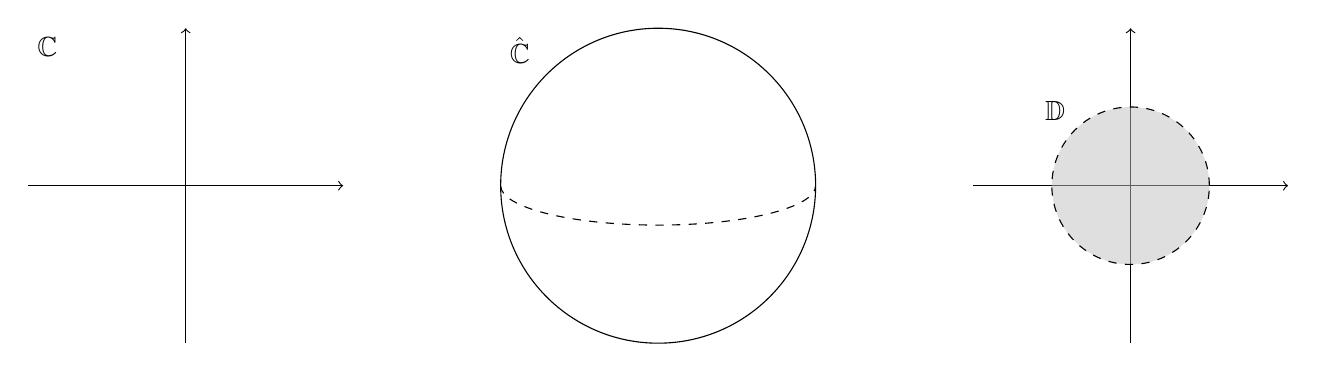
\begin{tikzpicture}
	\draw (0,0) circle (2);
	\draw[dashed] (-2,0) arc[start angle = 180, end angle = 360, x radius = 2, y
			radius = 0.5];
	\node[below right] at (current bounding box.north west) {$ \hat{\mathbb{C}} $};

	\begin{scope}[xshift=-6cm]
		\draw[->] (-2,0) to (2,0);
		\draw[->] (0,-2) to (0,2);
		\node[below right] at (current bounding box.north west) {$ \mathbb{C} $};
	\end{scope}

	\begin{scope}[xshift=6cm]
		\draw[->] (-2,0) to (2,0);
		\draw[->] (0,-2) to (0,2);
		\filldraw[dashed, fill=gray!50, fill opacity=0.5] (0,0) circle (1);
		\node[above left] at (135:1) {$ \mathbb{D} $};
	\end{scope}


\end{tikzpicture}
\end{document}
